%===============================================================================
% Debugging.
%===============================================================================

\section{Debugging}

\subsection{Debuging in general}

Why to (know how to) debug (huh ?)
\begin{itemize}
  \item eventually, every programmer will get to a point where there is
    a bug in his program which is non-obvious
    \begin{itemize}
    \item even with loads of testing (cannot simulate all real-life situations,
      hard to get 100\% code coverage in testing) \texttt{(3)}
    \item how to approach this problem in effective way ? (to find a root cause
      and correct fix)
    \end{itemize}
  \item debugging knowledge will make you to write the program with debugging
    in mind $\rightarrow$ leads to faster debug-fix-develop cycle \texttt{(2)}
  \item debugging is understimated, everyone seems to focus on programming
    techniques but not on how to find bugs in programs \texttt{(1)}
\end{itemize}

\begin{itemize}
  \item[(1)] and, some jobs are just about finding+fixing bugs.
  In pure development, surprisingly debugging skills
  often are not needed that much but when sustaining software it is crucial.
  \item[(2)] it is too late when developer realizes that the program contains
      horrendous amount of bugs but there is no debugging framework
      and logging capabilities are poor.
  \item[(3)] This is valid even for semi-real-life testing with
      eat-your-own-food test beds.
\end{itemize}

%===============================================================================
\subsection{Observing}

\begin{itemize}
  \item What to observe:
  \begin{itemize}
  \item system calls
  \item library calls
  \item transactions
  \item input/output data (e.g. network traffic)
  \item all of the above (ideally correlated/connected together)
  \end{itemize}
  \item How to observe:
  \begin{itemize}
  \item capture the events
  \item stop and run \texttt{(1)}
  \end{itemize}
\end{itemize}

\infoBox{Heisenbug}{
is special kind of bug named after Heisenberg's Uncertainty Principle -
altering the way program runs by observing it might make it harder to spot
a bug which depends on timing (race conditions etc.)
\url{http://en.wikipedia.org/wiki/Unusual\_software\_bug}
}

Special business (not covered):
\begin{itemize}
  \item kernel debugging
  \item performance debugging
\end{itemize}

%===============================================================================
\subsection{Helper tools}

\begin{itemize}
\item code browsing/exploring:
  \begin{itemize}
    \item useful for complex projects or areas you're not familiar with
    \item there are many tools, everyone has his own preference and work style
       (similar to code editors)
    \item web-based/terminal-based
  \end{itemize}
  \item getting information from binaries
  \item peeking into transient objects (processes, lwps, memory, ...)
\end{itemize}

%===============================================================================
\subsubsection{ctags}

\begin{itemize}
  \item easy to find definitions of functions/macros/variables
  \item very simple to use
  \item original ctags vs. exuberant ctags (\url{http://ctags.sourceforge.net/})
    \begin{itemize}
    \item limited number of supported languages (original: C, Pascal, Fortran)
    \item ectags better integrated with vim
    \end{itemize}
  \item how does it work: scans source code for definitions and generates
  $tag+file+regexp$ (\texttt{ex} command) for each definition found into
  \texttt{tags} file:
  \begin{verbatim}
  load_config  reload.c  /^int load_config(void) {$/
  \end{verbatim}
\end{itemize}

\begin{itemize}
  \item ctags examples:
  \begin{itemize}
  \item Emacs ctags:
\begin{verbatim}
  etags --declarations --defines --globals --typedefs *.[ch]
\end{verbatim}
  original \item original ctags:
\begin{verbatim}
  ctags *.[ch]
  ctags -R
\end{verbatim}
  \end{itemize}
  \item it will create output file called 'tags' and can immediately work
        with it
  \item vim setup: add the following into \texttt{~/.vimrc}:\\
  \texttt{set tags=./tags,./TAGS,tags,TAGS,/usr/inc{}lude/tags,~/Source/...}
  \item open vim and jump to the symbol: \\
     \texttt{vim -t known\_symbol}
  \item after that tab-complete via: \\
     \texttt{:ts symbolprefix}
  \item jump backwards via 'Ctrl-t'
  \item see tags stacks via \texttt{:tags}
\end{itemize}


%===============================================================================
\subsubsection{cscope}

\begin{itemize}
    \item great for caller/callee searching
    \item great for learning by observing code flow
      \begin{itemize}
      \item e.g. capture truss output (with multiple instances of -u) and 
        go through interesting functions
      \end{itemize}
    \item how does it work: generates index file (binary format) to
       \texttt{cscope.out} by going through the code (including header
       files)
    \item how-to for vim+cscope setup:
        \url{http://cscope.sourceforge.net/cscope\_vim\_tutorial.html}
\end{itemize}

\begin{itemize}
\item References:
\begin{itemize}
  \item cscope+ctags+vim setup:
     \url{http://www.fsl.cs.sunysb.edu/~rick/cscope.html}
  \item cscope+vim:
     \url{http://cscope.sourceforge.net/cscope\_vim\_tutorial.html}
\end{itemize}
\item Examples:
\begin{enumerate}
      \item find symbol definition:
        \begin{enumerate}
        \item produce \texttt{cscope.out} file:
        \texttt{cd \$SRC; cscope -b -R}
	  \begin{itemize}
	  \item some old implementations lack the -R recursive option: \\
	    \texttt{find . -type f -name '*.[ch]' > /tmp/list; cscope -b -i /tmp/list}
	  \end{itemize}
        \item in \texttt{vim} position the cursor over a symbol
        \item hit Ctrl-@ and 'g'
        \end{enumerate}
      \item search for a symbol
        \begin{enumerate}
        \item in \texttt{vim} position the cursor over a
            variable/function/definition
        \item hit Ctrl-@ and 's'
        \end{enumerate}
      \item find more about a function:
        \begin{enumerate}
        \item find a function definition via ctags \texttt{:ts func<tab>}
        \item see who calls this function 'Ctrl-@ + c'
        \end{enumerate}
\end{enumerate}
\end{itemize}

%===============================================================================
\subsubsection{OpenGrok}

\begin{itemize}
  \item source code search engine: \url{http://opengrok.github.io/OpenGrok/}
  \item cross-reference + syntax highlighting
    \begin{itemize}
    \item kind of similar to cscope but web-based
    \end{itemize}
  \item indexes most common languages (C, Java, ...)
    and SCMs (CVS, SVN, Mercurial, ...)
  \item allows to search based on definitions, symbols, paths, history, full
  search
  \item really fast (even with full search across many projects)
\end{itemize}

%===============================================================================
\subsubsection{Other tools}

\begin{itemize}
  \item \texttt{vimdiff}
    \begin{itemize}
    \item useful for comparing changes in source files or log files produced
      by different versions of the program in question
      \item even useful for watching changes in behavior
        (\texttt{truss} output)
      \item can be very useful in cases when we don't know what exactly
        has changed
    \item enable colored view via \texttt{:color on}
    \end{itemize}
  \item number of small tools like \texttt{bc, od, hexdump}, ...
  \item combinations
    \begin{itemize}
      \item e.g. combine dtrace/truss with graphviz and you'll get great
        call graphs:
          \url{http://thermalnoise.wordpress.com/2007/11/14/visual-call-graph-using-dtrace/}
    \end{itemize}
\end{itemize}

%===============================================================================
\subsection{Debugging data}

formats for embedding debugging information into ELF binaries

%===============================================================================
\subsubsection{stabs}

symbol table strings

\begin{itemize}
\item largely historical
\item debugging information is stored as special entries in symbol table
\end{itemize}

%===============================================================================
\subsubsection{DWARF}

\begin{itemize}
\item modern de-facto standard for representing debug data
\item large space overhead, difficult to process
\end{itemize}

XXX

\begin{itemize}
\item References:
  \begin{itemize}
  \item DWARF paper:
     \url{http://www.dwarfstd.org/Debugging\%20using\%20DWARF.pdf}
  \end{itemize}
\end{itemize}

% XXX pridat vic informaci o DWARF formatu, jak se s nim pracuje
% (tools pro nahlizeni apod.)

%===============================================================================
\subsubsection{CTF (Compact C Type Format)}

similar to DWARF in function but small space overhead (normally
used for all userland binaries and also kernel-land). Originally introduced in
Solaris, currently (2016) it is being added to FreeBSD.

\begin{itemize}
  \item stored in ELF section header called \texttt{.SUNW\_ctf}
  \item describes types, unions, typedefs, structures, function prototypes
  \item no binary to source code mapping
  \item manipulated by \texttt{ctfdump, ctfmerge, ctfconvert}, consumed by
    mdb(1), dtrace(1M)
  \item generated via -g compiler option from the stabs/DWARF data
    and replaces the data in the process (ctfconvert)
  \item Usually CTF is created from DWARF data
       % \item CTF format itself is described in XXX
\end{itemize}

References:
  \begin{itemize}
  \item On Solaris, CTF tools are available in the \texttt{onbld} package
  \begin{verbatim}
  pfexec pkg install developer/build/onbld
  export PATH=$PATH:/opt/onbld/bin:/opt/onbld/bin/`uname -p`
  \end{verbatim}
  \item \url{http://blogs.oracle.com/levon/entry/generating\_assembly\_structure\_offset\_values}
  \item \url{http://blogs.oracle.com/levon/entry/reducing\_ctf\_overhead}
  \item \url{https://blogs.oracle.com/jmcp/entry/getting_started_with_your_own1}
\end{itemize}

\Task{Construct library with CTF data}{debugging/ctf}{%
The data types supplied by the library can be described by CTF. The program
using the library does not necessarily have to support CTF for its data
structures. This task is Solaris/FreeBSD specific.}{%
\begin{itemize}
  \item Use \texttt{ctfconvert} and \texttt{ctfmerge} commands to supply CTF
    data to the library.
  \item Link a program with the library, call the \texttt{fillit()} function
    from the program. Use \texttt{ctfdump}, \texttt{elfdump} commands to verify
    the library indeed contains CTF data.
  \item Set a breakpoint at the entry to \texttt{fillit()} and
    verify the entry has been set
  \item Run the command in debugger, this time with a breakpoint set to the
    entry of the function \texttt{fillit()}
  \item print the contents of the structure with types and addresses/offsets
\end{itemize}
}

%===============================================================================
\subsection{Resource leaks}

\begin{itemize}
\item loose definition: resource leak is an event which happens when
   reference to a resource is removed without actually freeing the
   resource
\item Most common: \url{http://en.wikipedia.org/wiki/Memory\_leak}
  \begin{itemize}
  \item memory leak \texttt{(1)} is just one kind of resource leak
     - a process can also leak descriptors, objects/structures, files, ...
  \end{itemize}
\item Why it happens (in environment without garbage collector):
  \begin{itemize}
  \item oversight (insufficient analysis) / careless programming
  \item unexcersized code path or unexpected combination of configuration 
     options (testing/code coverage again), most commonly error paths
     \texttt{(2)}
  \end{itemize}
\end{itemize}

\begin{itemize}
  \item[(1)] by memory we mean the heap segment of a process.
  \item[(2)] "Snowball effect problem" (smallest possible case, imagine
  similar case with more allocations and complex dependencies):
\end{itemize}

\begin{lstlisting}
  /* pseudo-code */
  foo = malloc(sizeof (struct foo_t));
  /* foo needs to be processed first */
  if (process(foo) < 0) { /* failure */
        free(foo);
        return (-1);
  }

  bar = malloc(sizeof (struct bar_t));
  /* bar will be a clone of foo */
  if (clone(foo, bar)) < 0) { /* failure */
        /* GAH, something is missing here */
        free(bar);
        return (-1);
  }
\end{lstlisting}

%===============================================================================
\subsection{libumem}

\begin{itemize}
\item full-blown memory allocator (alternative to the allocator from libc)
\item suitable for debugging memory leaks \texttt{(1)}
\item minimal overhead (can be even used in production)
\item has pedigree of the slab allocator \texttt{(3)} (but in userland)
   \texttt{(2)}
\item no application modification necessary
  \begin{itemize}
  \item just LD\_PRELOAD the libumem.so library and set UMEM\_DEBUG environment
    variable
  \end{itemize}
\item scalable allocator (slabs) with memory debugging
  \begin{itemize}
  \item can diagnose memory leaks, double free's, used free'd memory etc.
  \end{itemize}
\end{itemize}

\begin{itemize}
\item[(1)] umem\_debug(3MALLOC) man page
\item[(2)] Per object type caches from which objects are allocated.
  Freeing of an object is a matter of returning it to the cache.
  If object constructors are used, the object is returned from the cache
  in initialized state and also must be returned to the cached in that state.
  For more details see the umem\_cache\_create(3MALLOC) man page.
\item[(3)] The Slab Allocator: An Object-Caching Kernel Memory Allocator
  (1994, USENIX), Jeff Bonwick
  \url{http://citeseerx.ist.psu.edu/viewdoc/summary?doi=10.1.1.29.4759}
\item References:
\begin{itemize}
  \item umem\_debug(3MALLOC)
  \item \url{http://blogs.oracle.com/ahl/entry/solaris\_10\_top\_11\_20}
  \item \url{http://blogs.oracle.com/jwadams/entry/debugging\_with\_libumem\_and\_mdb}
  \item \url{http://blogs.oracle.com/roller/page/jmcp?entry=on\_findleaks\_wot\_is\_it}
  \item \url{http://blogs.oracle.com/amith/entry/detecting\_memory\_corruption\_with\_libumem}
\end{itemize}
\end{itemize}

%===============================================================================
\subsubsection{How does libumem work}

\begin{itemize}
\item replacing default heap allocator in libc (preloading or directly
   linking against \texttt{libumem.so})
\item protecting the buffer with patterns which are checked inside
  libumem's malloc/free
  \begin{itemize}
  \item patterns:
    \begin{itemize}
    \item \texttt{0xbaddcafe} is free'd memory
    \item \texttt{0xdeadbeef} is uninitialized variables
    \item \texttt{0xfeedface} redzone (after the actual buffer contents)
    \end{itemize}
  \end{itemize}
\item recording the log of stack traces for each allocated buffer \texttt{(1)}
\item last piece: debugger going through global variables, 
   constructing reachability graph and finding unreachable addresses at
   the end
\end{itemize}

\begin{itemize}
  \item[(1)] makes it easy to identify who allocated that buffer
\end{itemize}

%===============================================================================
\subsubsection{Using libumem+mdb to find memory leaks}

\begin{itemize}
\item generic approach:
  \begin{itemize}
  \item run the program with preloaded \texttt{libumem.so} and environment
     variables which trigger special behavior of the library \\
     \texttt{LD\_PRELOAD=libumem.so UMEM\_DEBUG=default ./prog}
  \item attach debugger and use \texttt{::findleaks} to get memory leaks:
    \texttt{(2)}
\begin{verbatim}
  mdb -p <pid_of_prog>
  ::findleaks
\end{verbatim}
  \item get the stack trace history of leaked buffers via
      \texttt{::bufctl\_audit} \texttt{(3)}
  \end{itemize}
\item the view of the memory has to be consistent $\rightarrow$ need to
    have the program in quiescent state \texttt{(1)}
\end{itemize}

\begin{itemize}
  \item[(2)] alternatively, do it in one step: set the environment variables
      and run the program from the debugger, load libumem and stop it in
      a function:
\begin{verbatim}
  export LD_PRELOAD=libumem.so
  export UMEM_DEBUG=default
  mdb ./prog
  ::load libumem.so.1
  ::bp foobar
  :r <program_arguments>
\end{verbatim}
 \item[(3)] can get stack trace easily:
\begin{verbatim}
> ::findleaks
CACHE     LEAKED   BUFCTL CALLER
00076508       1 00097158 libc.so.1`strdup+0xc
------------------------------------------------------------------------
   Total       1 buffer, 24 bytes
> 00097158::bufctl_audit
            ADDR          BUFADDR        TIMESTAMP           THREAD
                            CACHE          LASTLOG         CONTENTS
           97158            91f48    6696e428fce34                1
                            76508                0                0
                 libumem.so.1`umem_cache_alloc+0x144
                 libumem.so.1`umem_alloc+0x58
                 libumem.so.1`malloc+0x28
                 libc.so.1`strdup+0xc
                 get_alg_parts+4
                 pluck_out_low_high+0x10
                 yyparse+0xe80
                 config_update+0x58
                 config_load+0x4c
                 main+0x474
                 _start+0x108
\end{verbatim}
  \item[(1)] Possible solutions:
  \begin{itemize}
    \item stop the program temporarily (\texttt{SIGSTOP} / Ctrl+Z)
    \item check for the leaks on the way to exit:

\begin{verbatim}
$ LD_PRELOAD=libumem.so
$ export LD_PRELOAD
$ UMEM_DEBUG=default
$ export UMEM_DEBUG
$ /usr/bin/mdb ./my_leaky_program
> ::sysbp _exit
> ::run
mdb: stop on entry to _exit
mdb: target stopped at:
libc.so.1`exit+0x14:    ta        8
mdb: You've got symbols!
mdb: You've got symbols!
Loading modules: [ ld.so.1 libumem.so.1 libc.so.1 ]
> ::findleaks
\end{verbatim}
    \item use gcore(1)
  \end{itemize}
\end{itemize}


%===============================================================================
\subsubsection{How does \texttt{::findleaks} work}

\begin{itemize}
  \item why is \texttt{::findleaks} needed at all ? wouldn't it be sufficient
     just to match \texttt{malloc()/free()} calls ? 2 disadvantages:
     \begin{itemize}
     \item space - necessary to log all the calls
     \item need to watch the process during whole life cycle \texttt{(1)}
     \end{itemize}
  \item \texttt{::findleaks} process:
  \begin{enumerate}
    % XXX overit a prozkoumat detailne
    \item start with static data
    \item grep memory for references to allocated blocks
  \end{enumerate}
\end{itemize}

\begin{itemize}
  \item[(1)] assumes the process has a cleanup routine which is run on the way
       to exit (e.g. server process which accumulates data over time).
\end{itemize}

\begin{itemize}
\item How does ::findleaks work
  \url{http://blogs.oracle.com/jwadams/entry/the\_implementation\_of\_findleaks}
\end{itemize}

\begin{itemize}
\item More tricks:
  \item \texttt{::umem\_debug}
    - enable debugging in libumem (umem\_debug())
  \item \texttt{::findleaks -f}
    - reinit full leak search (normally the results are cached)
  \item \texttt{::umem\_status}
    - shows heap corruptions in detail
\end{itemize}

\Task{Resource leak debugging}{debugging/resource-leaks/}{%
This piece of code resembles configuration reloading done in system daemons,
including errors.}{%
\begin{enumerate}
  \item See the source of \texttt{reload.c} and find all resource leaks.
  \item compile \\\texttt{make clean \&\& make}
  \item There are resource leaks happening during restart\\
  \texttt{kill -HUP `pgrep leaky`}
  \item Use your favorite tools to discover the resource leaks.
  \item Switch to different operating system and try to find the leaks
  with tools available there (preferably completely different tool chain).
  Compare the differences between various tools and approaches.
  \item Fix the leaks, use the tool to verify they are indeed gone.
\end{enumerate}
}

%===============================================================================
\subsection{watchmalloc}

\begin{itemize}
  \item Debugging library in Solaris similar to libumem, actually enforces
     the boundaries and correct memory allocation (i.e. detects double
     \texttt{free()}, write past the end of the buffer, etc.)
  \item has a mode which uses \texttt{/proc} watchpoint facility
     (\texttt{SIGTRAP} on invalid access)
     \begin{itemize}
     \item \texttt{WATCH}: free'd blocks are write protected
     \item \texttt{RW}: the area before and after the buffer (called
       \emph{red zone}) and free'd blocks are read/write protected
     \end{itemize}
\end{itemize}

\alertBox{The cost of debugging with watchmalloc}{has significant overhead
(even without watchpoints)}

~

\Task{watchmalloc experimentation and inspiration}{debugging/watchmalloc/}{%
The watchmalloc library can be used as inspiration for writing your own
heap allocator with detection capabilities.
}{%
\begin{enumerate}
  \item compile \\
    \texttt{make clean \&\& make}
  \item run with malloc from libc \\
    \texttt{./underoverflow 10 -2 16}
  \item run with watchmalloc and no write \\
    \texttt{LD\_PRELOAD=watchmalloc.so.1 MALLOC\_DEBUG=WATCH \
       ./underoverflow 10 -2 16}
  \item run with watchmalloc with read guards and write \\
     \texttt{LD\_PRELOAD=watchmalloc.so.1 MALLOC\_DEBUG=RW \
       ./underoverflow 10 -2 16 40}
  \item Experiment some more, try to read/write before the beginning of the
     buffer, etc. What is the granularity of detection ? Can watchmalloc detect
     off-by-one reads/writes ?
  \item test double free with watchmalloc \\
    \texttt{LD\_PRELOAD=watchmalloc.so.1 MALLOC\_DEBUG=WATCH ./badfree 10}
  \item Write your own simple heap allocator (using either \texttt{brk()} or
    \texttt{mmap()} with checking. Use \texttt{mprotect()} to protect metadata
    of each buffer. Implement double free detection.
  \item Produce unit tests for your allocator.
\end{enumerate}
}

\begin{itemize}
  \item References:
  \begin{itemize}
  \item \url{http://blogs.oracle.com/wfiveash/entry/playing\_with\_solaris\_memory\_debuggers}
  \item \url{http://blogs.oracle.com/peteh/entry/hidden\_features\_of\_libumem\_firewalls}
  \item \url{http://blogs.oracle.com/eschrock/entry/watchpoints\_features\_in\_solaris\_10}
  \end{itemize}
\end{itemize}

%===============================================================================
\subsection{Call tracing}

\begin{itemize}
  \item syscalls: truss(1)/strace(1)
  \begin{itemize}
    \item both work across fork(2) with \texttt{-f}
  \end{itemize}
  \item library calls: truss(1)/ltrace(1) \texttt{(3)} \texttt{(4)}
    \begin{itemize}
    \item to observe calls to functions in the executable \texttt{(1)}
    \end{itemize}
  \item invasive observation: both truss and strace stop the program for a while
  \item how does it work: manipulate with lwp via the \texttt{/proc}
     interface \texttt{(2)}
\end{itemize}

% XXX add short explanation how truss works (it is just a interpreter)

\begin{itemize}
  \item[(1)] Example: get all calls done by functions in \texttt{nc} binary
  and also by functions from \texttt{libc.so} library which have
  \texttt{get} prefix:
\begin{verbatim}
truss -u a.out -u libc::get* nc www.mff.cuni.cz 80
\end{verbatim}
  \item[(2)] truss uses \texttt{libproc.so} to access \texttt{/proc}.
  \item[(3)] truss can trace also library calls:
\begin{verbatim}
  truss -f -ulibcrypto::pk11_* -upkcs11_softtoken:: \
      `pgrep traced-app` > /tmp/app.truss 2>\&1
\end{verbatim}
  \item[(4)] trace calls in the program itself: \texttt{truss -u a.out}
  \item note on \texttt{truss} and its data representation. If you truss a
  ``hello world'' program, you will see something like this at the end:

\begin{verbatim}
Hello world.
write(1, " H e l l o   w o r l d .".., 13)      = 13
_exit(0)
\end{verbatim}

  Ie., you see spaces within the strings. The thing is that \texttt{truss} needs
  2 characters to represent a byte. It uses hexadecimal representation for
  non-printable cha\-rac\-ters, ascii for printables chars, and escapes where
  possible ($\backslash$\texttt{n}, $\backslash$\texttt{r}, etc.). So, if you
  print three characters: 0x01, the new line character (0x0a), and X (0x58),
  you will see this:

\begin{verbatim}
write(1, "01\n X", 3)                          = 3
\end{verbatim}
\end{itemize}

~

\Task{Construct your own strace}{debugging/ptrace/strace.c}{%
\texttt{strace}/\texttt{truss} basic functionality can be constructed using
\texttt{/proc} or \texttt{ptrace()} interfaces. Getting the syscall number
and return code is architecture dependent, it is necessary to find out where
(e.g. in which registers) the data is stored.
}{%
\begin{enumerate}
\item Adapt the source code to trace system calls of a program. The output
should include syscall number and return code, i.e. something like this: \\
\texttt{syscall \#21 called} \\
\texttt{syscall \#21 returned with 0}
\end{enumerate}
}

%===============================================================================
\subsection{Using /proc}

\begin{itemize}
  \item p-commands (proc(1)):
     \begin{itemize}
     \item pstack
     \item pfiles
     \item pcred
     \item pldd
     \item pmap 
     \end{itemize}
  \item Exmaple: check for file descriptor leaks:
  \begin{enumerate}
    \item stop the process \texttt{(1)} via pstop(1)
    \item watch the open descriptors via pfiles(1)
    \item see the stack via pstack(1)
    \item continue the run via prun(1)
    \item jump to step nr. 1
  \end{enumerate}
\end{itemize}

\begin{itemize}
  \item[(1)] p-commands can operate on LWPs and core files
\end{itemize}

Example:

\begin{verbatim}
    $ sleep 20 \&
=====> remember the PID
    [1] 7407
=====> stop the process
    $ pstop 7407
=====> wait a bit too see it's really stopped
    $ sleep 20
=====> see the userland stack
    $ pstack 7407
=====> unbrake the process again
    $ prun 7407
\end{verbatim}

\begin{itemize}
\item How does it work ?
  \begin{itemize}
  \item via proc(1). Use the above example with: \\
    \texttt{truss pstop 7407}
  \item NOTE: pstop(1) can even stop a single lwp
  \end{itemize}
\end{itemize}

\begin{itemize}
\item References:
  \begin{itemize}
  \item pfiles can display filenames:
  \url{http://blogs.oracle.com/eschrock/date/20040712#nuts\_and\_bolts\_of\_pfiles}
  \item \url{http://blogs.oracle.com/ahl/entry/the\_solaris\_10\_top\_111}
  \item pmap can display libraries and regions for thread stacks:
  \url{http://blogs.oracle.com/ahl/entry/number\_18\_of\_20\_pmap}
  \end{itemize}
\end{itemize}

%===============================================================================
\subsection{Debugging dynamic libraries}

\begin{itemize}
  \item ld.so.1(1)
  \item Run-time linker and link-editor have shared built-in debugging
  capability: \\
  \texttt{LD\_DEBUG=help /bin/ls}
\end{itemize}

Example: using \texttt{LD\_DEBUG}: \\
\begin{verbatim}
  LD_DEBUG=symbols,bindings /usr/bin/openssl speed \
    rsa1024 -engine pkcs11
\end{verbatim}

\begin{itemize}
  \item Note: can use ld.so.1 for running a program:
\begin{verbatim}
  /lib/ld.so.1
  /lib/ld.so.1 /bin/ls
  /lib/64/ld.so.1 /bin/ls
  /lib/64/ld.so.1 /usr/bin/amd64/openssl version
\end{verbatim}
\end{itemize}

%===============================================================================
\subsection{Debuggers}

\begin{itemize}
  \item Kinds of debuggers:
  \begin{itemize}
    \item generic - able to debug both userland/kernel (gdb/mdb/adb)
    \item in-kernel (kmdb)
    \item userland (dbx)
  \end{itemize}
  % XXX http://www.logix.cz/michal/doc/article.xp/debug-1
  \item How userland debugger works:
  \begin{itemize}
     \item ptrace(3C) / proc(4) \texttt{(1)}
     \begin{itemize}
       \item start/stop: \texttt{PCSTOP} et al., \texttt{PCRUN}
       \item single stepping: \texttt{PRUN} + \texttt{PRSTEP}
       \item breakpoints: \texttt{PCWRITE} with trap instruction \texttt{(2)}
       \item watch points: \texttt{PCWATCH}
       \item read/write process memory: \texttt{PCREAD/PCWRITE}
     \end{itemize}
  \end{itemize}
\end{itemize}

\begin{itemize}
  \item[(1)] ptrace() is just a proc(4) wrapper in Solaris, regular
     syscall in Linux (ptrace(2))
% \url{http://src.opensolaris.org/source/xref/onnv/onnv-gate/usr/src/cmd/mdb/common/mdb/mdb\_proc.c#proc\_ops}
  \item[(2)] \texttt{0x91d02001} for SPARC, \texttt{0xcc} for i386/AMD64,
%    \url{http://src.opensolaris.org/source/xref/onnv/onnv-gate/usr/src/lib/libproc/common/Pcontrol.h#BPT}
%    \begin{itemize}
%    \item Breakpoint setting is done via \texttt{libproc.so} in
%    \url{http://src.opensolaris.org/source/xref/onnv/onnv-gate/usr/src/lib/libproc/common/Pcontrol.c#Psetbkpt}
%    \end{itemize}
  \item References: Crash dump analysis lecture (NPRG050)
     \url{http://dsrg.mff.cuni.cz/teaching/nprg050/}
\end{itemize}

%===============================================================================
\subsection{Symbol search and interposition}

\begin{itemize}
\item default model symbol search can be quite complicated
\item Symbol search:
\begin{itemize}
  \item each reference to the symbol by given object leads to a search
  \item first found instance wins
  \item ldd(1) reports the order in which the search will be done
  \item each symbol search starts from the application
\end{itemize}
\item Interposition:
\begin{itemize}
  \item foo() definition in bigfoo.so.1 interposes on foo() definition 
    in smallfoo.so.1
\end{itemize}
\end{itemize}

Example: \priklad{debugging/symbol-search/}
\begin{enumerate}
    \item see thee source files and try to guess:
       \begin{itemize}
       \item which functions from which files will be called ?
       \item what will happen ?
       \item how many times we lookup symbol 'bar' ?
       \end{itemize}
    \item compile \\
       \texttt{make clean \&\& make}
    \item observe the library dependencies:
\begin{verbatim}
       ldd ./prog
       ldd ./bigbar.so.1
\end{verbatim}
    \item run: \\
       \texttt{./prog}
    \item see what happened: \\
       \texttt{LD\_DEBUG=symbols,bindings ./prog}
\end{enumerate}

% XXX produce better image
%\begin{center}
%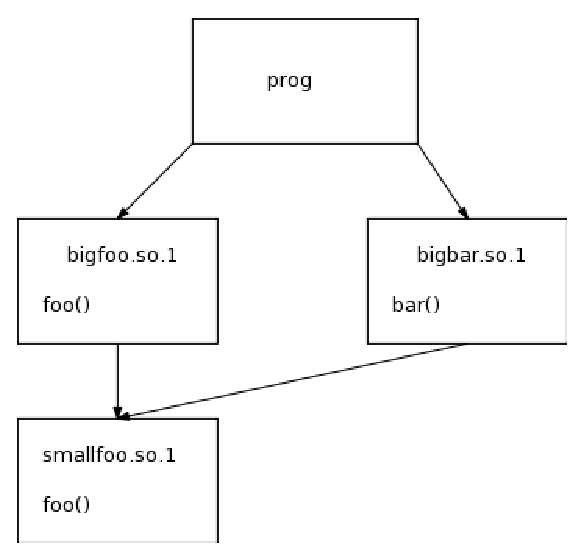
\includegraphics[width=60mm,keepaspectratio]{img/debugging/symbol-search.eps}
%\end{center}

%===============================================================================
\subsection{dtrace}

\begin{itemize}
\item dynamic instrumentation
\item ...
\item Available on: Solaris, FreeBSD, Mac OS X, QNX
\item performance/lock contention debugging
\end{itemize}


\begin{itemize}
\item References:
  \begin{itemize}
  \item dtrace guide
  \item The Solaris Dynamic Tracing (DTrace) Guide:
  \item dtrace(1M) man page
  \end{itemize}
\end{itemize}

\endinput
